\section{Introducción}

El aprendizaje por refuerzo es un paradigma de aprendizaje automático en el que un agente aprende a tomar decisiones interactuando con un entorno y recibiendo recompensas o penalizaciones.

Este trabajo se centra en la implementación y evaluación experimental de tres algoritmos de aprendizaje por refuerzo en el entorno \textit{CliffWalking-v0}, de la librería de Python \textit{Gymnasium}, con el objetivo de comparar su rendimiento y eficiencia en dicho entorno. Los algoritmos implementados son: \textit{Value Iteration}, \textit{Direct Estimation} y \textit{Q-Learning}.

\subsection{Caracterización del entorno}

El entorno de \textit{Cliff Walking}, propuesto originalmente por \textit{Sutton \& Barto}, es un entorno clásico para evaluar algoritmos de aprendizaje por refuerzo. En este entorno, el agente debe navegar por una cuadrícula de dimensiones 4x12 evitando caer en un acantilado, lo que representa una penalización significativa. El objetivo del agente es llegar a la esquina inferior derecha de la cuadrícula de la forma más eficiente posible, maximizando la recompensa acumulada a lo largo del tiempo y minimizando el número de pasos necesarios para alcanzar la meta.

\begin{figure}[h]
    \centering
    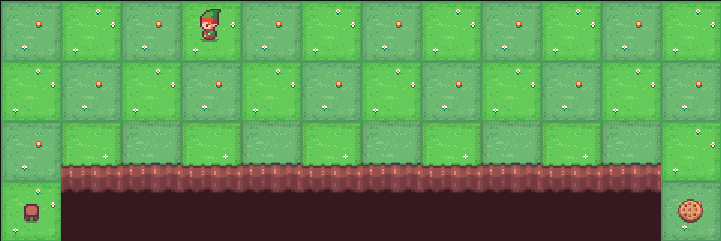
\includegraphics[width=0.7\textwidth]{images/mapa.png}
    \caption{Captura de pantalla del entorno \textit{Cliff Walking}. El agente comienza en la esquina inferior izquierda (s0) y debe llegar a la esquina inferior derecha (sT), evitando caer en el acantilado (cliff) representado por las celdas marrones.}
    \label{fig:cliff-walking-map}
\end{figure}

A continuación se caracteriza de forma detallada el entorno:

\begin{itemize}
    \item \textbf{Observabilidad}: Totalmente observable. El agente recibe en cada paso su posición exacta en la cuadrícula, sin ruido ni información oculta, por lo que tiene acceso total al estado relevante.
    \item \textbf{Número de agentes}: Un único agente.
    \item \textbf{Determinismo}: Estocástico, ya que está activado el modo \texttt{is\_slippery=True}. En este caso, por cada acción que el agente toma, hay una probabilidad de aproximadamente el 66.7\% de que el agente se resvale hacia una dirección perpendicular a la acción deseada.
    \item \textbf{Atomicidad}: Secuencial. Las decisiones del agente tienen consecuencias que dependen de toda la historia de acciones y percepciones, y los efectos futuros de las acciones importan para maximizar la recompensa acumulada.
    \item \textbf{Dinamicidad}: Estático. El estado del entorno sólo cambia cuando el agente toma una acción; no hay cambios “por sí mismos” mientras el agente razona.
    \item \textbf{Continuidad}: Discreto. Tanto el espacio de estados (posiciones en la cuadrícula) como el de acciones (arriba, abajo, izquierda, derecha) y el tiempo de decisión son discretos.
    \item \textbf{Conocimiento}: Conocido. Las reglas de transición (aunque estocásticas) y la función de recompensa están definidas de antemano y son accesibles al agente.
\end{itemize}

\subsubsection{Espacio de acciones}

El agente dispone de un conjunto finito de acciones
\[
  \mathcal{A} = \{\text{Arriba},\, \text{Derecha},\, \text{Abajo},\, \text{Izquierda}\},
\]
cada una de las cuales intenta desplazar al agente una celda en la dirección indicada.

\subsubsection{Estados inicial y terminal}
\begin{itemize}
  \item \textbf{Estado inicial} $\;s_0=(3,0)$, correspondiente a la esquina inferior izquierda de la cuadrícula.
  \item \textbf{Estado terminal} $\;s_T=(3,11)$, la meta en la esquina inferior derecha; al llegar aquí, el episodio termina.
\end{itemize}

Si durante el episodio el agente cae en el acantilado, este regresa al estado inicial $s_0$ y continua con el episodio.

\subsubsection{Función de recompensa}
La señal de recompensa $R(s,a,s')$ se define como:
\[
  R(s,a,s') = 
  \begin{cases}
    -100, & \text{si } s' \text{ es una celda de acantilado (cliff),}\\
    -1,   & \text{en cada transición válida que no alcance la meta ni el cliff,}\\
    \;0,  & \text{al alcanzar el estado terminal } s_T.
  \end{cases}
\]
De este modo, el agente está incentivado a llegar cuanto antes a la meta evitando caer en el precipicio.


\subsection{Entorno experimental}

\begin{table}[H]
  \centering
  \begin{tabular}{@{} ll @{}}
    \toprule
    \textbf{Componente} & \textbf{Descripción} \\
    \midrule
    Sistema operativo      & Ubuntu 24.04.2 LTS \\
    Kernel Linux           & 6.10.3-061003-generic \\
    CPU                    & AMD Ryzen 7 5825U (8 núcleos, 16 hilos, hasta 4.5\,GHz) \\
    GPU integrada          & AMD Radeon Graphics (Barcelo) \\
    Memoria RAM            & 16\,GB DDR4 \\
    Intérprete de Python   & Python 3.\,9.\,18\quad \\
    \bottomrule
  \end{tabular}
  \caption{Entorno de hardware y software utilizado en los experimentos}
  \label{tab:entorno-experimental}
\end{table}